\documentclass[twoside]{article}
\usepackage{amsgen,amsmath,amstext,amsbsy,amsopn,amssymb,}
\usepackage{graphicx}
\usepackage{epsfig}

\setlength{\oddsidemargin}{0.1 in} \setlength{\evensidemargin}{-0.1 in} 
\setlength{\topmargin}{-0.6 in} \setlength{\textwidth}{6.5 in}
\setlength{\textheight}{10.4 in} \setlength{\headsep}{0.1 in}
\setlength{\parindent}{0 in} \setlength{\parskip}{0.1 in}

\newcommand{\homework}[2]{
   \pagestyle{myheadings}
   \thispagestyle{plain}
   \newpage
   \setcounter{page}{1}
   \noindent
   \begin{center}
   \framebox{
      \vbox{\vspace{2mm}
       \hbox to 6.28in { {\bf Math 1700:~Elementary Statistics \hfill} }
       \vspace{6mm}
       \hbox to 6.28in { {\Large \hfill #1 (#2)  \hfill} }
       \vspace{6mm}
      \vspace{2mm}}
   }
   \end{center}
   \markboth{#1}{#1}
   \vspace*{4mm}
}

\newcommand{\bbF}{\mathbb{F}}
\newcommand{\bbX}{\mathbb{X}}
\newcommand{\bI}{\mathbf{I}}
\newcommand{\bX}{\mathbf{X}}
\newcommand{\bY}{\mathbf{Y}}
\newcommand{\bepsilon}{\boldsymbol{\epsilon}}
\newcommand{\balpha}{\boldsymbol{\alpha}}
\newcommand{\bbeta}{\boldsymbol{\beta}}
\newcommand{\0}{\mathbf{0}}

\begin{document}

\homework{$1^{st}$ Week Summary}{09/01/23}
\vspace{-.4in}
\begin{itemize}
\setlength\itemsep{0em}
\item Algebra review:
\subitem Summation: 
\subsubitem $\sum_{i=1}^nx_i=x_1+x_2+\cdots+x_n$
\subsubitem $\sum_{i=1}^nx_i^2=x_1^2+x_2^2+\cdots+x_n^2$
\subsubitem $\left(\sum_{i=1}^nx_i\right)^2=\left(x_1+x_2+\cdots+x_n\right)^2$
\subsubitem $\sum_{i=1}^nx_iy_i=x_1y_1+x_2y_2+\cdots+x_ny_n$
\subitem Factorials: 
\subsubitem $n!=n\times (n-1)\times\cdots 2\times 1$
\subitem Computations:
\subsubitem e.g. $x+y\dfrac{\sqrt{s}}{n}$
\subitem Solving simple linear equations:
\subsubitem $2-2x=3x+3$
\item What is statistics?
\item Descriptive statistics vs Inferential statistics.
\item Population vs Sample.
\item Variables and Data values.
\item Parameter vs Statistic.
\item Two types of data: 
\subitem Qualitative [Nominal and Ordinal] 
\subitem Quantitative [Continuous and Discrete]
\item Sampling Techniques
\subitem Simple Random Sample (SRS)
\subitem Stratified Random Sample
\subitem Cluster Sample
\item Ways to chart qualitative data: Bar graphs and Pie charts
\item Ways to chart quantitative data: Dot plot, Stem and Leaf plot, and Histogram

\item Measures of Central Tendency
\subitem Mean: $\bar{x} = \dfrac{x_1+x_2+\cdots+x_n}{n} = \dfrac{\sum_{i=1}^nx_i}{n}$
\subitem Median:
\subsubitem If n odd, $\tilde{x}=$ middle value
\subsubitem If n even, $\tilde{x}=$ average of middle two values
\subitem Mode: The value that happens most often in sample
\subitem Midrange $ = \dfrac{L+H}{2}$

\item Measures of Dispersion
\subitem Range $ = H - L$
\subitem Sample Variance: $s^2=\dfrac{1}{n-1}\sum_{i=1}^n(x_i-\bar{x})^2=\dfrac{1}{n-1}\left\{\sum_{i=1}^nx_i^2-\dfrac{\left(\sum_{i=1}^n x_i\right)^2}{n}\right\}=\dfrac{1}{n-1}SS(x)$
\subitem Sample Standard deviation: $s=\sqrt{s^2}$

\begin{figure}[h]
\vspace{-4.8in}
\hspace{3.5in}
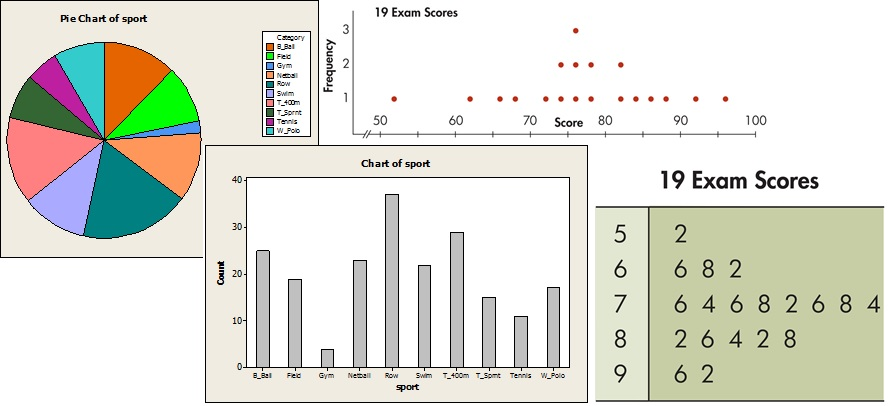
\includegraphics[angle=0,width=3in] {../graphs.jpg}
\end{figure}

\end{itemize}
\end{document}
